The system is used primarily to identify certain patterns in different types of multivariate time-series. In this section, we highlight several examples -  three real world datasets and a synthetically generated dataset.  We also briefly describe some applications of the system.  The models based on the three presented datasets can be found on the StreamStory website (\url{http://streamstory.ijs.si}). 


%\lstopar{
%The experiment was conducted by simulating the characteristic curve (linear characteristics) of a typical direct current permanent magnet electric motor \cite{book:1107411}.
%}

\subsection{Weather Data}
\label{sec:experiments-weather}
This is dataset represents monthly rainfall and temperature data
collected over the course of 20 years between 1920 and 1940 in Nottingham, \primoz{England\cite{}}. 
The resulting model can be seen in Figure~\ref{fig:example-weather}. 

\begin{figure}[h!]
	\centering
	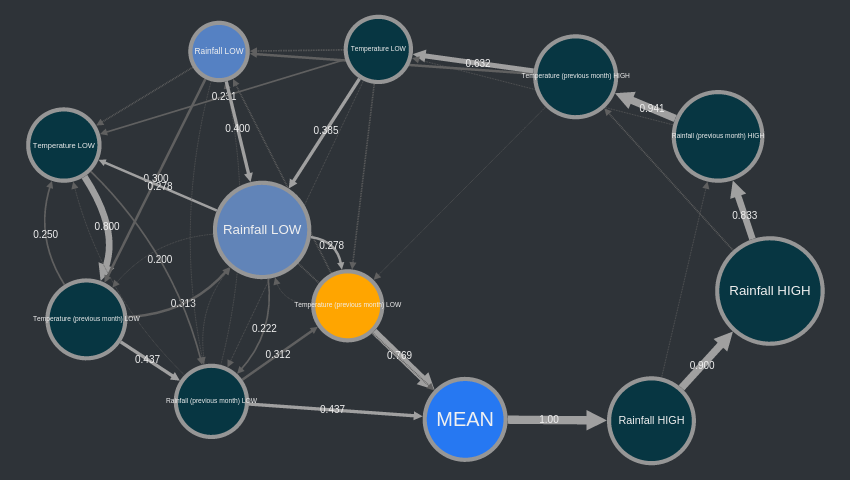
\includegraphics[width=\columnwidth]{example-weather}
	\caption{Qualitative representation of temperature and rainfall data collected over the course of 20 years. The yearly timeline flows in the clockwise direction with the right-most state representing the summer, the bottom states representing autumn, the left-most states representing winter and the top states representing spring.}
	\label{fig:example-weather}
\end{figure}

The model was generated using the raw rainfall and temperature data. This two dimensional dataset was first  lifted into a four dimensional space. This was done using the values of the current month and previous month as the four coordinates.
By appending the previous sample to the current sample, effectively adding two new dimensions. This is a basic version of a time-delay \primoz{embedding~\cite{}} to obtain a better embedding of the data into Euclidean space.

First, we see the yearly cycle represented as a cycle in the graph of the Markov chain. 
The states on the right hand side represent the 
summer states, while the states on the left represent winter states. The yearly timeline flows in the clockwise direction with the spring states residing on the bottom of the figure and the autumn
states on the top.

Interestingly, in this dataset, the rainfall and temperature are highly correlated and the automatic labeling service
chose high rainfall as the most significant feature of the summer states. This correlation can be seen
from the histograms in Figure \ref{fig:histograms-summer}.

Using our model, we can clearly see how the summer and winter dynamics differ. While the summer states seem quite deterministic, with a high probability of jumping into the next state in the clockwise direction, the transition probabilities in the winter states are much more uniform, suggesting larger fluctuations in the weather during the winter.

\begin{figure}[h!]
	\centering
	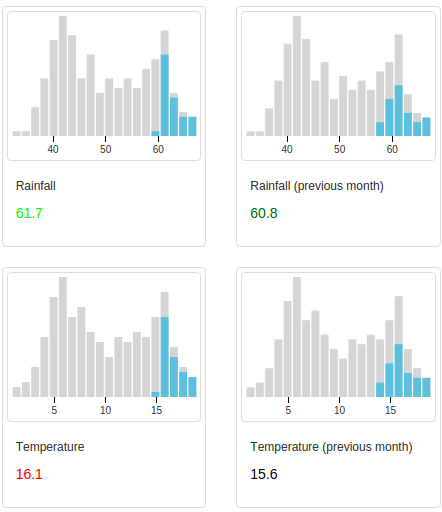
\includegraphics[width=0.7\columnwidth]{histograms-summer}
	\caption{Histograms of all the attributes in one of the summer states of the weather example shown in Figure \ref{fig:example-weather}. The histograms suggest a high correlation of temperature and rainfall.}
	\label{fig:histograms-summer}
\end{figure}

\subsection{GPS Data}

The second example was created using raw GPS coordinates collected using a smartphone between years 2012 and 2015.
The data represents the everyday movement of a European computer science researcher. Figure \ref{fig:example-geo}
shows our qualitative representation of this data on a high level with $9$ states.

\begin{figure}[h!]
	\centering
	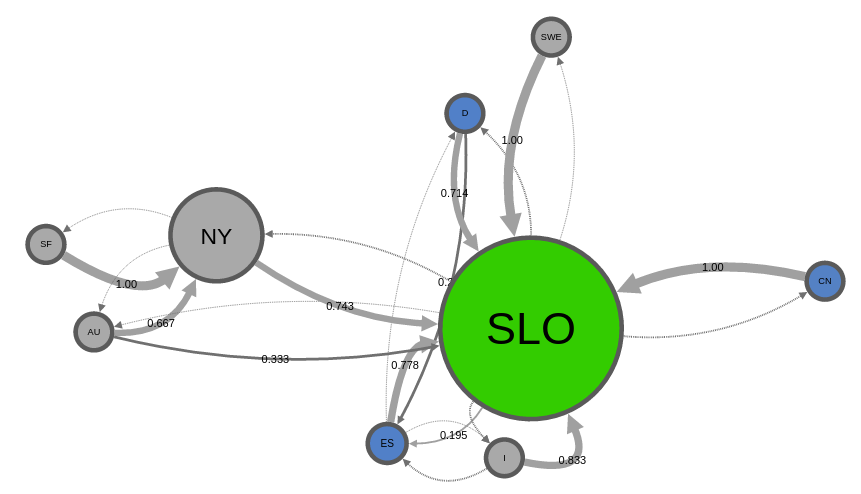
\includegraphics[width=\columnwidth]{geo-states}
	\caption{Qualitative representation of GPS data representing the movements of a European researcher, collected over the course of four years. Using our system, we were able to identify the most typical locations where the person traveled, including the USA, Germany, Italy, Spain, Sweden, China and Slovenia, their associated states are shown labeled using appropriate country/city codes.}
	\label{fig:example-geo}
\end{figure}

We can see that the system was able to identify the most typical locations of this persons
movements. The researcher spent most of their time in the large green state representing Slovenia. On the European continent, the system was able to identify Germany, Sweden and Spain where the person frequently attends meetings as well as Italy, which represents a common transition state airport. The small state on the right is China, where they vacationed in 2015. The states on the left represent the USA with the largest of the three representing New York city where the person spent the 2014 summer and the smaller two states representing San Francisco and Austin, Texas.

The system identified the coordinates of these locations, whereas the naming was done manually.

\subsection{Traffic Data}

Our final real-world example, shown in Figure \ref{fig:example-traffic-multiscale}, shows a multi-scale representation of two traffic counters positioned on a highway ring around Ljubljana, Slovenia. The time series is the number of cars per hour passing each counter, sampled every hour.  Here we again lifted the dataset into a four dimensional space by appending the reading from three hours in the past to the current reading.

\begin{figure}[h!]
  	\centering
  	\begin{subfigure}[b]{.48\columnwidth}
	  	\centering
	  	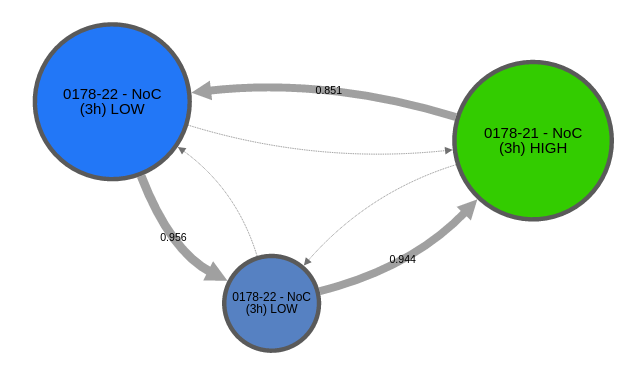
\includegraphics[width=\columnwidth]{traffic-coarcest}
  		\caption{\label{fig:traffic-coarcest}}
	\end{subfigure}
  	\begin{subfigure}[b]{.48\columnwidth}
	  	\centering
	  	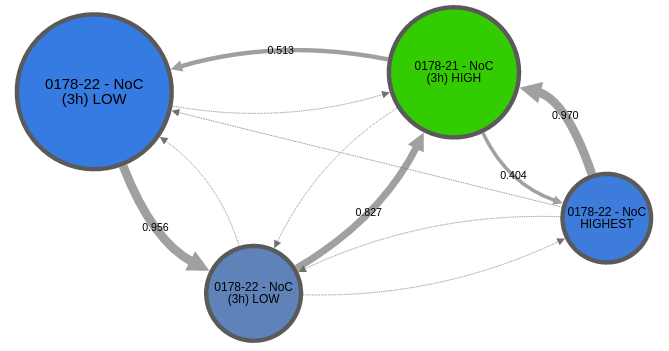
\includegraphics[width=\columnwidth]{traffic-coarcer}
  		\caption{\label{fig:traffic-coarcer}}
	\end{subfigure}
	\begin{subfigure}[b]{.48\columnwidth}
	  	\centering
	  	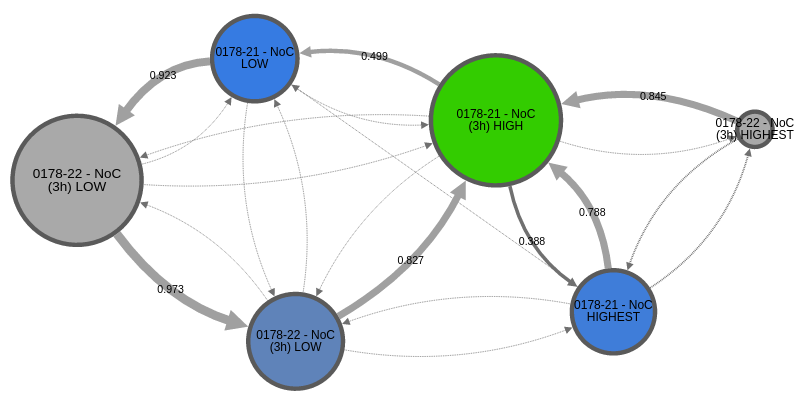
\includegraphics[width=\columnwidth]{traffic-middle}
  		\caption{\label{fig:traffic-middle}}
	\end{subfigure}
	\begin{subfigure}[b]{.48\columnwidth}
	  	\centering
	  	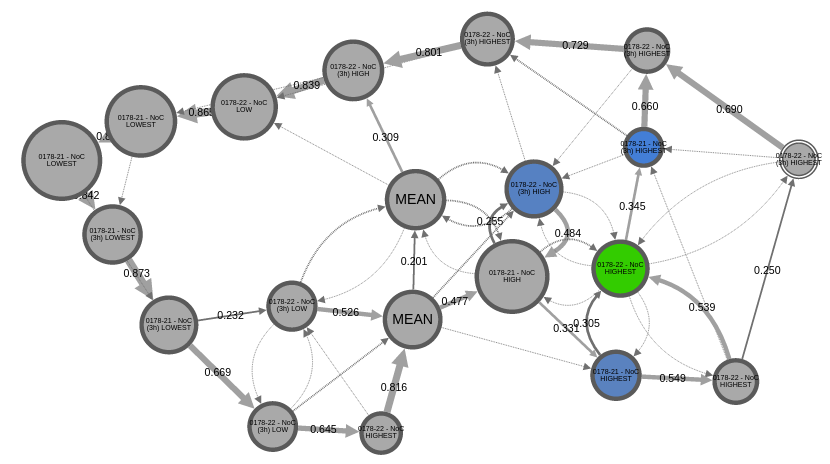
\includegraphics[width=\columnwidth]{traffic-finest}
  		\caption{\label{fig:traffic-finest}}
	\end{subfigure}
  	\caption{A multi-scale representation of two traffic counters positioned on Ljubljana's highway ring from a coarse scale \ref{fig:traffic-coarcest} down to the finest scale \ref{fig:traffic-finest}. From our model we identified what we believe is the typical daily cycle on the ring flowing in the counter clockwise direction. On the finest scale in Figure \ref{fig:traffic-finest} one can clearly distinguish the nightly and daily dynamics with the nightly dynamics being very deterministic while various events introduce much noise in the day time.}
  	\label{fig:example-traffic-multiscale}
\end{figure}

\begin{figure*}[th!]
  	\centering
  	\begin{subfigure}[b]{.48\textwidth}
	  	\centering
	  	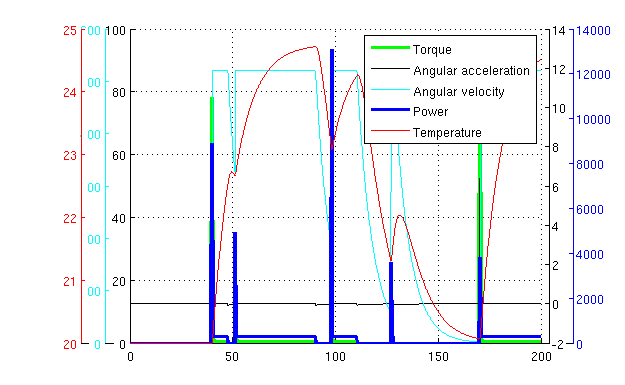
\includegraphics[width=\columnwidth]{simulation-processed}
  		\caption{\label{fig:simulation-chart}}
	\end{subfigure}
  	\begin{subfigure}[b]{.48\textwidth}
	  	\centering
	  	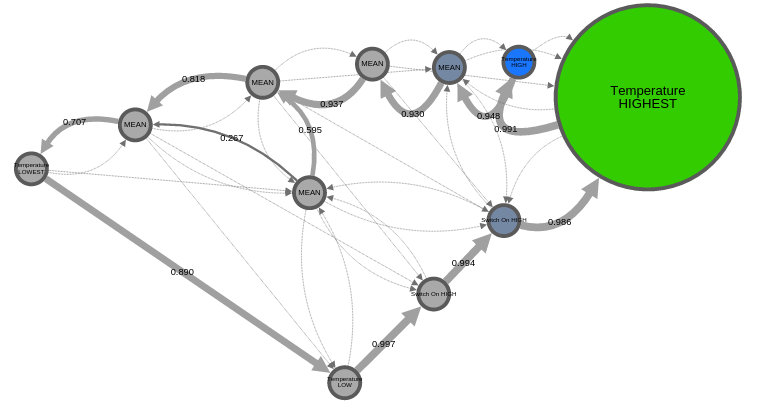
\includegraphics[width=\columnwidth]{model-motor-simulated}
  		\caption{\label{fig:simulation-model}}
	\end{subfigure}
  	\caption{Simulation of an electric motor plotted as a standard time-chart \ref{fig:simulation-chart} and our qualitative model \ref{fig:simulation-model}. We see the cyclical behavior of the motor warming up to the large state on the upper right and then subsequently cooling down. }
  	\label{fig:example-motor}
\end{figure*}

On a coarse scale with only three states, we were able to identify the typical daily cycle on the ring. The cycle starts with the leftmost state in Figure~\ref{fig:traffic-coarcest} representing the night state with a low number of cars detected by both sensors lasting from approximately $9$PM to $6$AM. It then moves in the counter clockwise direction into the bottom state representing the morning. The morning state has a relatively high number of cars detected on both sensors, lasting from $7$ to approximately $9$AM. The state on the right of Figure~\ref{fig:traffic-coarcest} represents the day state lasting from $10$AM to approximately $9$PM.

When zooming into a finer scale, shown in Figure \ref{fig:traffic-coarcer}, the rightmost state is split in two. The top-left of the two new states (green) now represents noon and evening and has a moderate number of cars, averaging $907$ and $631$ cars per hour for the two counters respectively. From this state, the system moves either back into the night state or into the afternoon state on the right of Figure \ref{fig:traffic-coarcer} with the highest number of cars detected on both sensors, with an average of $1240$ and $1290$ cars per hour. This state lasts from approximately $3$PM to $6$PM when the system jumps back into the moderate day state.



When zooming even further into Figure \ref{fig:traffic-middle}, interestingly, the system detects a small state which typically occurs on Friday evening and is shown on the right of Figure~\ref{fig:traffic-middle}. This is the time when most of the students leave the city and go home for the weekend and when people in general leave for weekend trips.

Zooming even further in Figure~\ref{fig:traffic-finest}, each state now represents a small time interval with the nighttime states in the top left of the figure and the daytime states on the bottom right. We can clearly see the more deterministic transitions in the nighttime states  and the larger variation in the daytime states, due to significantly higher traffic during the day.
%It is not surprising that the transitions in the nightly states seem a lot more deterministic than in the daily states. Indeed, at night not a lot of cars drive on the ring while during the day various events introduce noise into the system.

% \primoz{
% \begin{itemize}
% \item Here we also need some examples of where its not useful -  a few different scales and we need references on the data. These can be deliverables. 
% \item Also we should show how much information we lose over different scales.
% \end{itemize}}


\subsection{Synthetic Data}
We also tested our system on a synthetic dataset,
simulated the heating patterns of a direct current permanent magnet electric motor \cite{book:1107411} using its typical characteristic curve. %simulating the characteristic curve (linear characteristics) of a typical direct current permanent magnet electric motor \cite{book:1107411}. 
This allowed us to validate the computed model as well as test its predictive power.  
The computed model is shown in Figure~\ref{fig:example-motor}. 

The simulation begins in the leftmost state of Figure~\ref{fig:simulation-model} with the motor in a stationary state
and the power switch turned off. Randomly, sampled from an exponential distribution, a switch is flipped to turn the motor on. Once the switch is on, as the rotation increases, the model starts moving in the counter clockwise
direction towards the large green state on the right. This state represents equilibrium when the temperature
gained through friction equals the temperature lost to the ambient and the signals become stationary.
Once the power switch is flipped to off, the rotation slowly halts due to friction and the process goes from right to
left in the counter clockwise direction. 

We generated two datasets: a training set and a test set, both containing $200k$ observations. The model was computed with 20 initial states on the training set using two attributes: angular velocity and temperature. Then on the testing data, before the process jumped, we extracted the next state probabilities and predicted the next state as the state with the highest probability.
We then computed the prediction accuracy as the ratio between the number of correct predictions and the total number
of jumps (total number of predictions). This serves as a check of the validity of our model. The model scored $0.845$. We also tried created a model which included a signal from the logical switch signal, raisign the score to $0.904$.

These experiments represent reality check for our approach rather than a rigorous evaluation, where we have a complete understanding of the underlying data. 
%Comparing the models' jump chain $\Pi$ and the . %The training dataset was then replayed and the initial states stored. We then used

%the stored states to calculate the transition probabilities and compared them to the models' jump chain $\Pi$. Since a lot of these probabilities were zero, we only used the probabilities that
%are non-zero either in the jump chain or in the probabilities calculated from the history. We then
%computed the mean absolute error of the non-zero probabilities which resulted in $MAE=0.05$ or $5\%$.

% To test the model's predictive power, we built  two models: (a) one 
% using the same attributes as in the first experiment, while in the second model (b), we used
% the logical switch signal to model state transitions. The models were trained on the same dataset
% as in the first experiment. Before the process jumped, we extracted the next state probabilities
% and used the state with the highest probability as the predicted next state. We then computed
% the prediction accuracy as the ratio between the number of correct predictions and the total number
% of jumps (total number of predictions). In this experiment model (a) scored $0.845$ while model
% (b) scored $0.904$.

\subsection{Domain Experts}
In the above examples, the discovered states could be interpreted by non-experts. We have also tested the system in more specialized settings. One example the system was tested on measurements from an oil drilling platform\footnote{Unfortunately, at the time of submission, we were not cleared to share the results of the analysis, including an evaluation on useability.}. In this data, natural recurrent behaviour was detected.  The model also detected an ``event,'' where certain equipment failed and drilling needed to be halted.  

%A second example is based on a manufacturing plant. In this case, we cannot 

